\documentclass[titlepage]{article}

\usepackage[english]{babel}
\usepackage[a4paper, left=3cm, right=2cm, top=2.5cm, bottom=3cm]{geometry}
\usepackage{amsmath}
\usepackage{graphicx}
\usepackage{placeins}
\usepackage[table]{xcolor}
\usepackage[colorlinks=true, allcolors=blue]{hyperref}
\usepackage[acronym]{glossaries}
\usepackage[parfill]{parskip}

\bibliographystyle{IEEEtran}
\graphicspath{{figures/}}
\makenoidxglossaries

\newacronym{qut}{QUT}{Queensland University of Technology}
\newacronym{gpu}{GPU}{Graphics Processing Unit}
\newacronym{api}{API}{Application Program Interface}
\newacronym{wgsl}{WGSL}{WebGPU Shading Language}
\newacronym{sdf}{SDF}{Signed Distance Function}

\begin{document}

\begin{center}
    
\includegraphics[scale=0.75]{Extension.pdf}
\end{center}

\begin{titlepage}
    \begin{center}
        \vspace*{7cm}

        \Huge
        \textbf{Creating a Voxel Rendering Engine}

        \vspace{0.5cm}

        \Large
        EGH400-1 Progress Report - Semester 2, 2022

        \vspace{0.25cm}

        \large
        Supervised by Professor Clinton Fookes

        \vspace{0.5cm}

        \Large
        \textbf{Alex McDermott (N10494367)}

        \vfill

        \Large
        The Queensland University of Technology\\
        \today
    \end{center}
\end{titlepage}

\tableofcontents
\listoffigures
\printnoidxglossary[type=\acronymtype]
\newpage

\section{Current Circumstances}
I'd like to preface this report with a summary of the current circumstances. Creating a voxel engine has only been the focus of this thesis for just under three weeks now. Up until Week 10, another student and I were working on a different topic which was supposed to be an industry connection with Airbus. Sadly, they were unable to follow through on their promise and representative to manage the project on their end so this arrangement fell through. Fortunately, our \acrfull{qut} supervisor Professor Clinton Fookes, has been very accommodating towards this jarring series of events so late in the semester. As a result of this, my current project is a student-led idea that I pitched as an alternative that will be more feasible due to the greatly reduced time frame. I chose this topic as I have experience with similar rendering techniques such as ray marching and feel that this somewhat familiar field coupled with my interest in the topic will aid in making up for the lost time.

\section{Project Summary}
The goal of this thesis project is to create a voxel rendering engine. Traditionally, rendering has been done with the use of triangles. These triangles are connected together in varying densities and sizes to create 3D models. They are then projected from 3D space to the 2D camera plane, and through a process called rasterization, the pixels they occupy are shaded. To begin understanding how voxel rendering differs from this we must first define what a voxel is. A voxel is a cell of a 3D grid where each cell stores information about the density at its particular location in space. Essentially a 3D pixel. Due to its innate ability to store this density data, it is commonly used in medical imaging as an output data structure for Magnetic Resonance Imaging and Computed Tomography scans. Another use for voxels is in video games where they can be used to implement destructible terrain such as in Teardown \cite{teardown:steam}. This thesis aims to create a program that can render these objects interactively in real time with lighting and shading effects.

\section{Interim Deliverables}
\subsection{Language Choice}
Rendering is generally a very computationally expensive process no matter the algorithm that is being used. This is due to the sheer amount of data that needs to be processed/created to produce an image of a usable size. Most displays these days output images at a minimum of 1080p meaning 1920 pixels wide by 1080 pixels high. For a renderer creating one of these images, this alone is already two million pixel colour calculations that are likely being performed at least 30 times per second in a real-time application. Observing the need for performance in creating a real-time rendering application, it was clear an efficient language would be needed. Due to this consideration, I chose Rust to make this application. It's a modern, fast, memory-safe, low-level language with performance comparable to C although with a significantly more pleasant developer experience. Rust ranked number one on the list of most loved languages in the most recent StackOverflow Developer Survey \cite{survey}, and with such an active community, has a wide array of high-quality packages readily available. Also, due to this language's overwhelming popularity, there is a wealth of educational resources available to aid in development.

\subsection{Wgpu}
Despite having chosen a sufficiently fast programming language above, implementing a real-time rendering engine that runs entirely on the Central Processing Unit is just not feasible. To accomplish this project we will be taking advantage of the \acrfull{gpu} which is able to process many pixels in parallel, thus improving computation times per frame by orders of magnitude. Although, there are many different \acrshort{gpu} hardware architectures and \acrfull{api} options, making it impractical to target all of them as a single developer. Because of this, it is common to use an abstraction layer such as Wgpu \cite{wgpu:source}, which I opted to use here, that handles the communication between these platforms under the hood. Wgpu is a Rust library that implements the WebGPU \cite{webgpu} \acrshort{api}, meaning it exposes a single set of methods that give us the ability to run natively in Vulkan, Metal, DirectX, and OpenGL graphics environments.

Having decided on a language and graphics \acrshort{api} it was time to begin getting content drawn to the screen. I began this process by following the Learn Wgpu \cite{wgpu:tutorial} tutorial. This walked through the process of setting up a Rust project with the required dependencies, as well as instantiating a window for the application with a basic event loop. Given this window object, a few more components are required before we can obtain a visual output. Firstly an adapter is created which handles interactions with the graphics card and provides information such as its name, backend, and power preference. The adapter can then be used to create a surface which is the part of the window that's drawn too. Having this level of control over the graphics process means operations such as resizing and updating the window dimensions need to be kept performed manually so this was also implemented here.

With these key components created I can now explain the \acrshort{gpu} pipeline. These are the steps the graphics system takes to go from a set of vertices, to an image on the screen. In this simple case, we are just looking to get up and running so I started with a single triangle. Next, a buffer, meaning a contiguous location of memory on the \acrshort{gpu}, was created to hold the required vertices for our primitive shape. This can be seen in the figure below along with the colours assigned to each vertex.

\begin{figure}[htp]
    \centering
    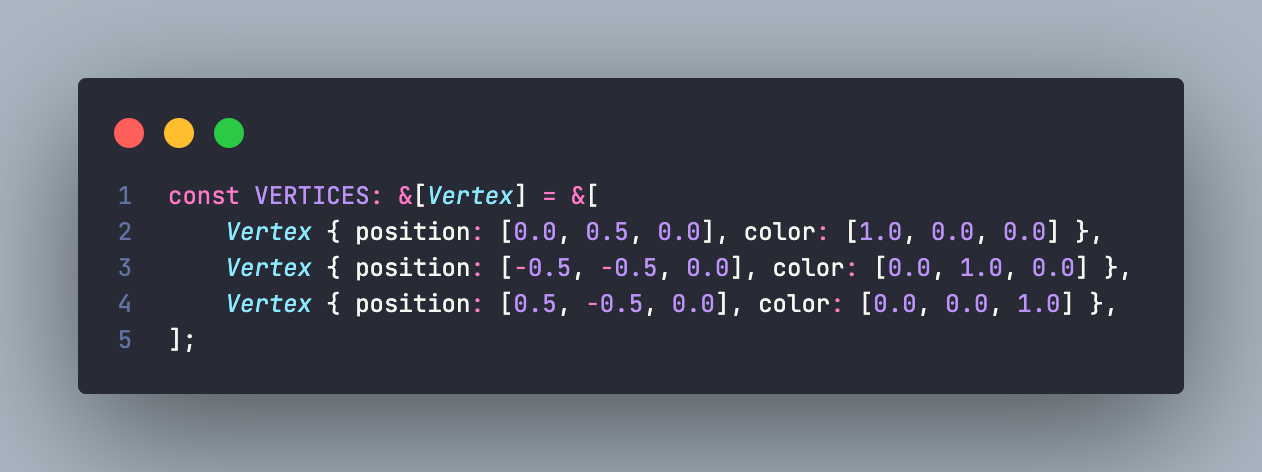
\includegraphics[width=0.75 \textwidth]{triangle_vertices.png}
    \caption{Definition of vertices and colours written to the \acrshort{gpu} buffer.}
\end{figure}
\FloatBarrier

This data is then passed into our pipeline, which in the case of Wgpu is handled by the \acrfull{wgsl}. Due to the simplistic nature of our shader, no processing is required on this vertex data and since the colours are already included, they can be extracted and used in the fragment shader with a small amount of code. This results in the image seen in the figure below.

\begin{figure}[htp]
    \centering
    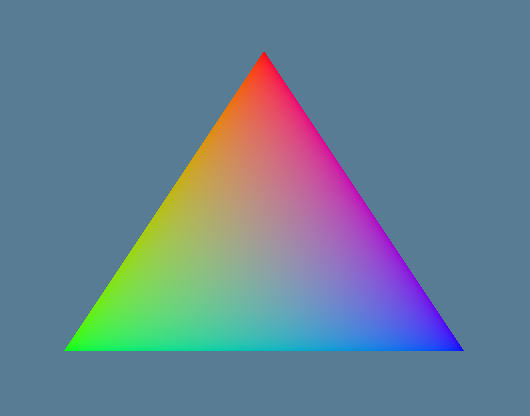
\includegraphics[width=0.5\textwidth]{coloured_triangle.png}
    \caption{Single triangle coloured using vertex colours.}
\end{figure}
\FloatBarrier

\subsection{Ray Marching}
Moving on from the basic Rust \acrshort{gpu} rendering proof of concept explored above, it was time to get familiar with the semantics of \acrshort{wgsl}. Having experience with the older OpenGL Shading Language, I was interested in figuring out the similarities and differences so I could apply my existing knowledge to this new system. To do this, my idea was to implement a basic but familiar ray marching render. A benefit of this was that the fundamentals of ray marching are quite similar to that of voxel rendering so I was hopeful some code, as well as knowledge, would be transferable. Building off the triangle that was currently being rendered, the colour data was stripped out and an extra vertex was added to create a rectangle that filled the whole screen. The reasoning for this was that ray marching is a software technique, it could be entirely implemented in the fragment shader. Each pixel of the image could be calculated separately and displayed on a single full-screen rectangle.

Discussing the technical details of ray marching, the whole premise is based on a function that returns the distance to the closest object in the scene given any sample point. This function is referred to as a \acrfull{sdf}. For each pixel, a ray is sent out at an angle determined by the field of view. The \acrshort{sdf} is then sampled to determine the minimum safe distance the ray can be marched before intersecting with an object. This process is repeated until the \acrshort{sdf} returns a value less than some threshold, indicating an object has been hit, or reaches some set number of maximum iterations indicating the opposite. This concept is visualised particularly well in the figure shown below.

\begin{figure}[htp]
    \centering
    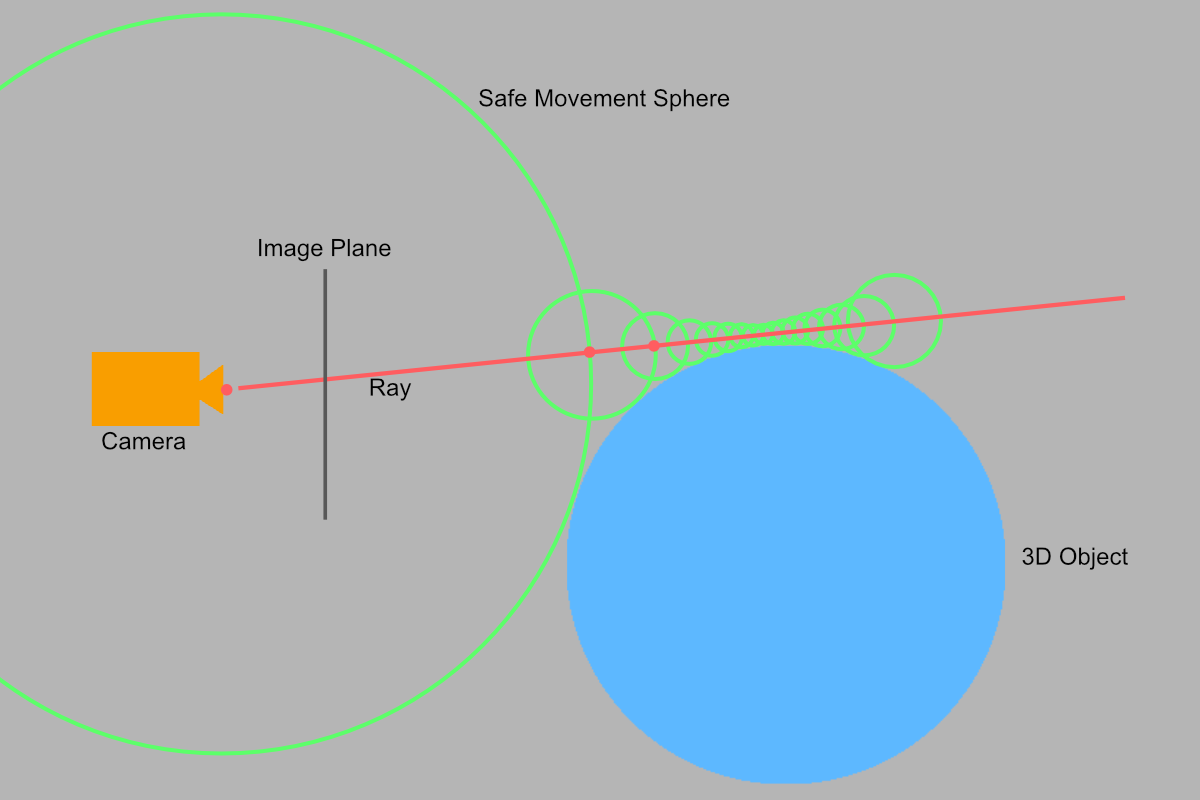
\includegraphics[width=0.7\textwidth]{ray_marching.png}
    \caption{Illustration demonstrating the concept of ray marching.}
\end{figure}
\FloatBarrier

The process described here was implemented in the fragment shader of our graphics pipeline. For each pixel, if a hit was detected, the gradient of the \acrshort{sdf} was found by calculating the differences between two samples a small distance apart. This gradient was used as the basis for Phong shading \cite{phong} which allows the sphere below to be visualised with approximated diffuse lighting and specular highlights.

\begin{figure}[htp]
    \centering
    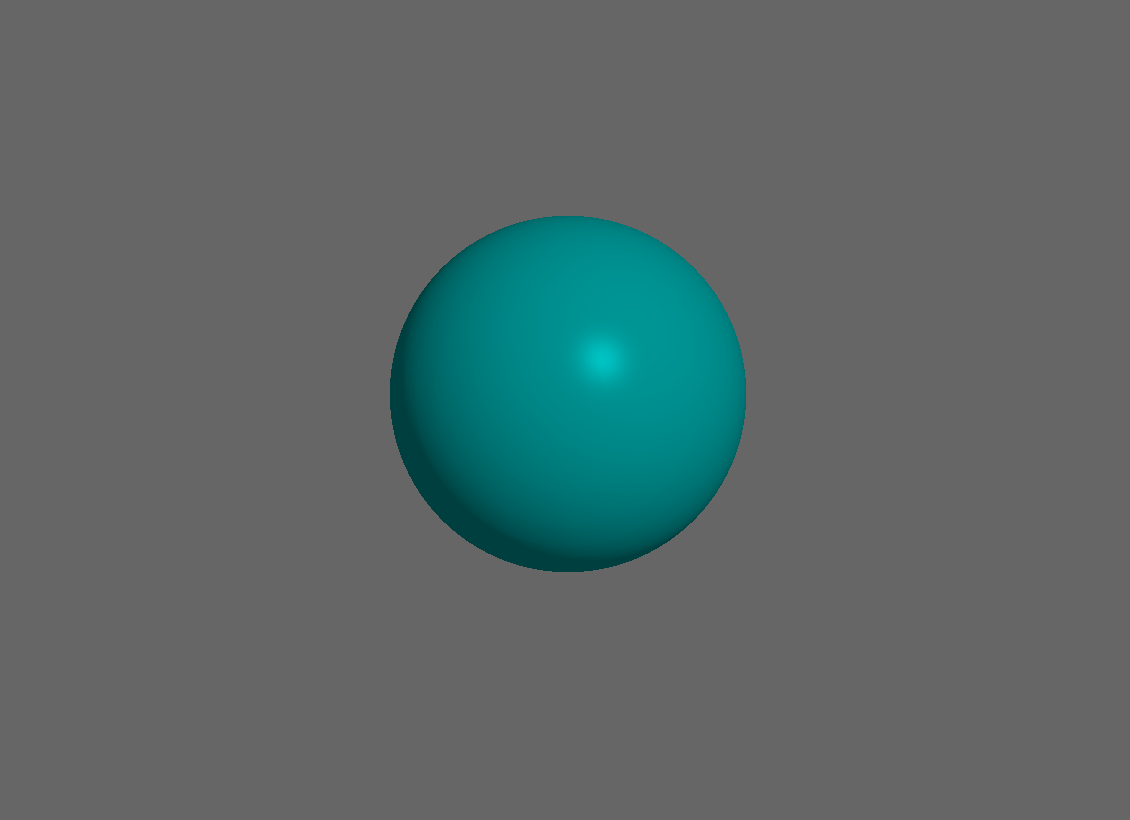
\includegraphics[width=0.5\textwidth]{phong_shading.png}
    \caption{Ray marched sphere using Rust and Wgpu.}
\end{figure}
\FloatBarrier

\subsection{Bevy}
Observing the output of the above sections, the result is quite desirable. It provides us with a means of writing shader code for our \acrshort{gpu} pipeline and visualising the output. Although, there were several steps involved in reaching this point, primarily all the manual interfacing with the Wgpu library which created a large amount of boilerplate code. My concern with this was that, as our application grows more complex, these more manual processes would take more and more time from actual engine development. To combat this, I decided to make the switch to a very popular Rust game engine called Bevy \cite{bevy}. Bevy is a data-driven game engine that uses an Entity Component System which has become a common approach in recent years. Even early on the benefits of this switch would be apparent, allowing for the removal of all of the Wgpu boilerplate code. Very conveniently, Bevy comes with plugins for window creation, event loops, and rendering primitives, out of the box. It also has a system in place for writing custom shaders for objects which we will be using extensively. This switch would allow us to focus on writing the actual shader code instead of micro-optimising the \acrshort{gpu} surfaces, buffers, etc. Further utilising the prospering Rust package ecosystem, I was able to import an open-source first-person flying camera controller \cite{flycam}. This was would prove to be very helpful as it would allow for debugging of vector maths with relation to object and camera positions. With less than 50 lines of code using the Bevy ECS system, we can create the basic 3D scene as shown below as opposed to the hundreds required previously to draw a single quad using Wgpu.

\begin{figure}[htp]
    \centering
    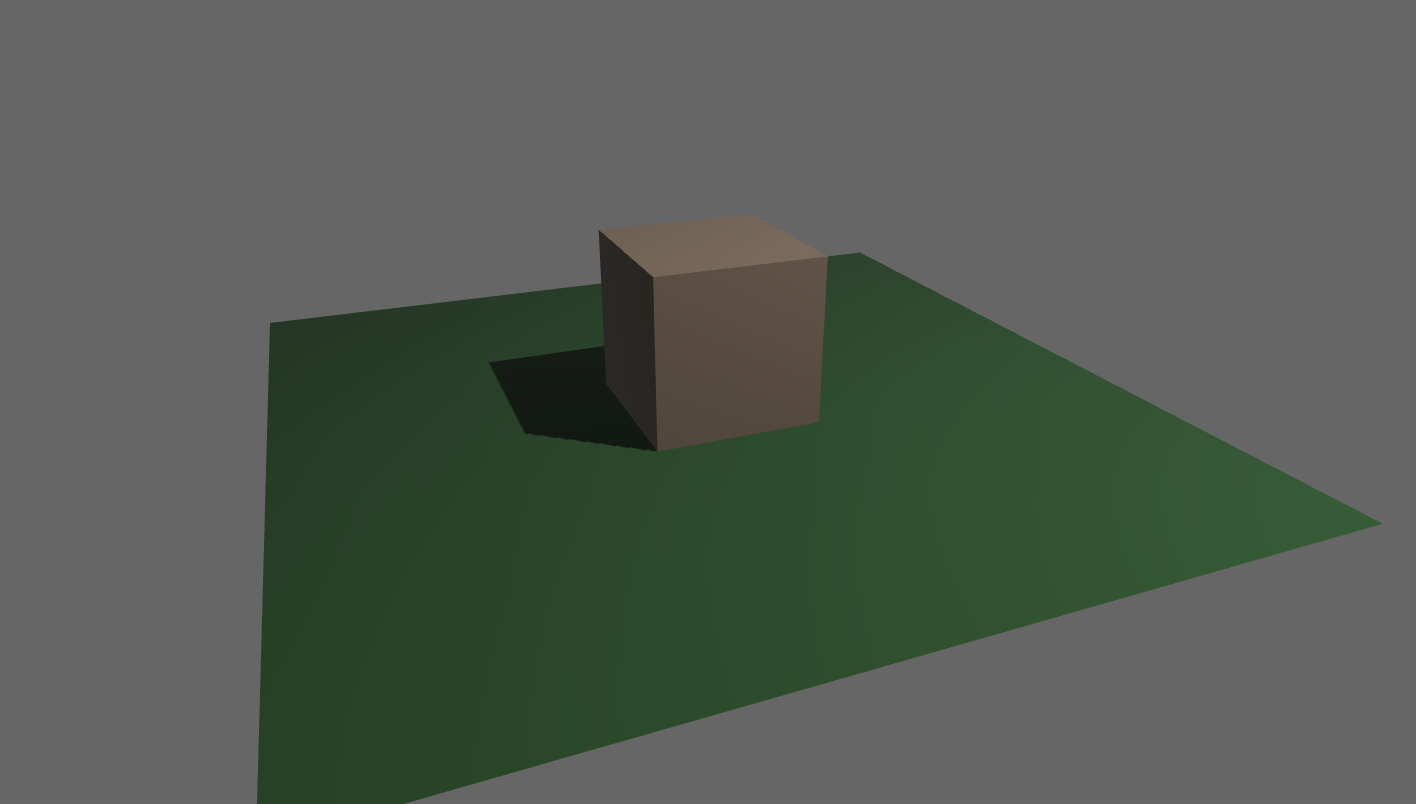
\includegraphics[width=0.75\textwidth]{bevy.png}
    \caption{Basic 3D scene created with Bevy.}
\end{figure}
\FloatBarrier

Having now switch libraries, I was interested in porting over the shader code I previously wrote for Wgpu. Fortunately, both libraries are quite progressive in terms of shader language choice and supported \acrshort{wgsl}. This made bringing over the bulk of the shading code quite simple as only the ray directions needed to be recalculated. Having watched a video by the Tuxedo Labs team on the technical aspects of their game Teardown \cite{teardown:tech}, I saw how they used cube meshes to render voxel volumes. This was also a reason behind the switch to Bevy as with the new system, it would be much easier to create many cube meshes if required in the future. This could allow for a scene to be composed of multiple voxel volumes without manually specifying all the vertex buffers, etc. In terms of converting our code to render our ray marched sphere on the texture of a cube, as stated, the ray direction would need to be recalculated. It was found that this could be done by accessing the points' 3D world position from within the fragment shader and then subtracting the position of the camera. The result of this "projection" of the ray marched sphere onto the cube gives the illusion of a volume as that is effectively what is being simulated. Shown below is the result of this process, the black cube outline can easily be hidden but is left in to enhance understanding.

\begin{figure}[htp]
    \centering
    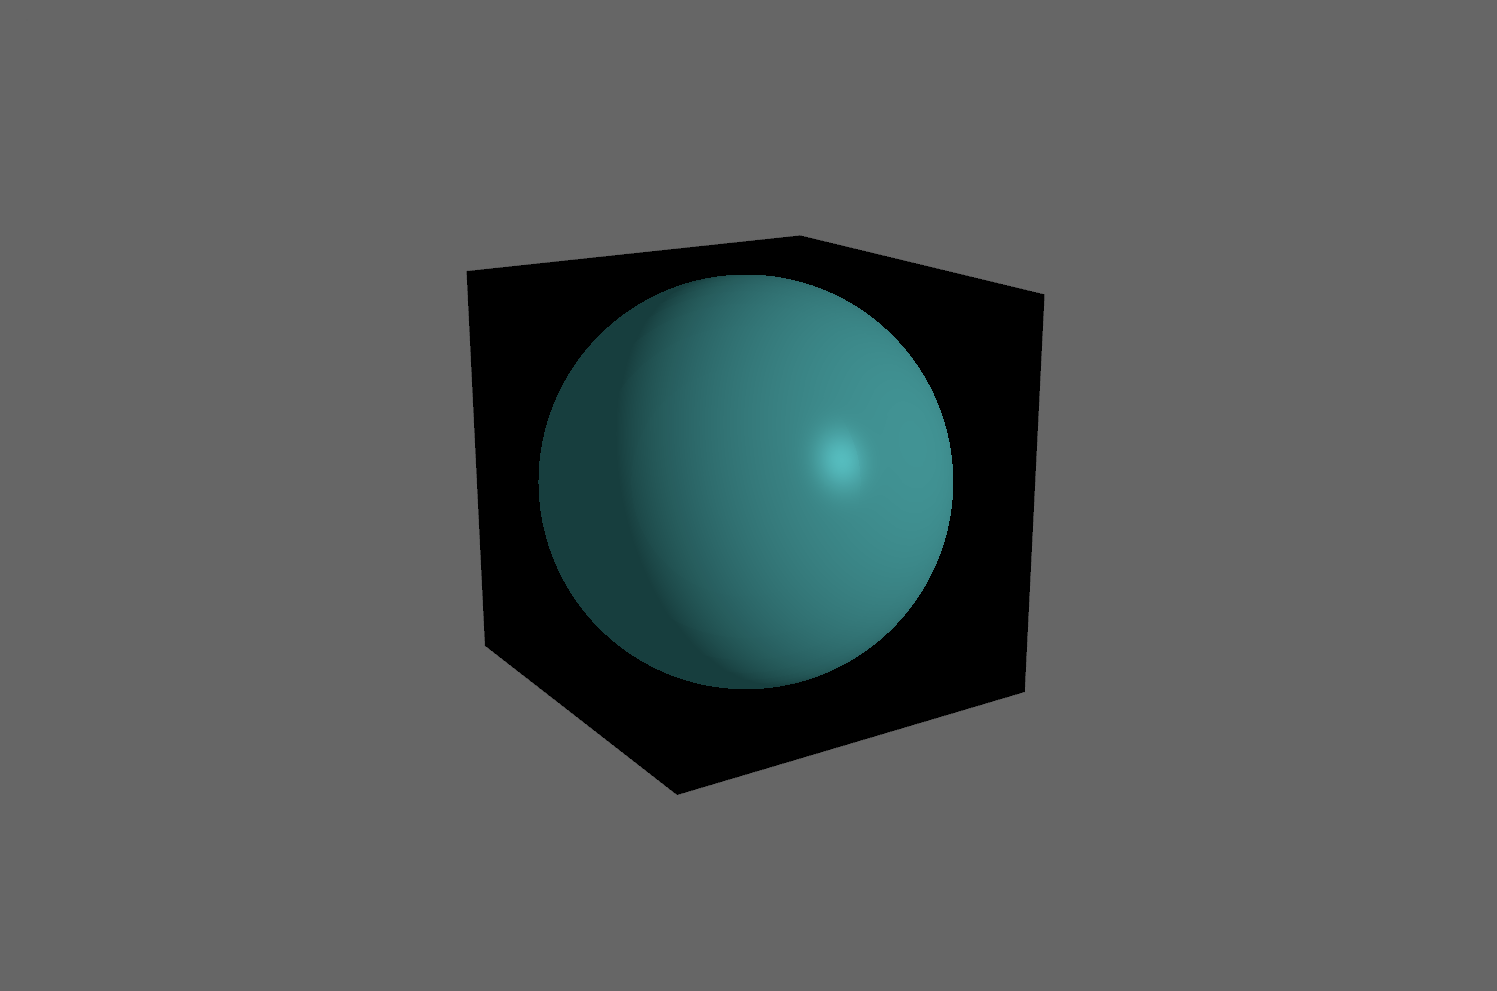
\includegraphics[width=0.75\textwidth]{cube.png}
    \caption{Ray marching shader on a cube, giving the illusion of a volume.}
\end{figure}
\FloatBarrier

\section{Risk Management}
Thankfully, being a software application, there is a negligible chance of physical risks associated with this project. Despite this, there are still some minimal data-related risks present which have been accounted for as follows. Data stored in a single place can be susceptible to loss from hardware failure or by misplacing the physical device. To combat this, Git version control has been used to both keep track of incremental program changes on a line-by-line basis, as well as keep a cloud-based backup through the GitHub service \cite{github}. Another crucial aspect that must be considered when working on a programming project is the data involved and the security and privacy expected when handling it. In the case of this voxel engine, there is no sensitive currently being handled. There is a chance that this could change in the future if the application is given the ability to read medical data. If this happens I will be sure to implement it professionally and utilise security best practices.

\section{Ethical Considerations}
Ethics are an important consideration when completing any project. For Engineers, we must look to the Engineers Australia Guidelines \cite{ethics} to aid in our professional conduct. Firstly, regarding codes 1.1, 1.3, 3.1, and 3.3, in summary, one must act in good conscience, respect dignity, uphold trustworthiness, and honestly communicate. This has been upheld throughout this project via diligent citation and referencing of a vast number of helpful resources, giving credit where credit is due. The codes described competent practising under section 2 which has also been upheld by my continued effort to stay up to date with the constantly evolving field of software and technology. I do this out of passion but also in the interest of always striving to produce a clean, maintainable software solution that follows best practices.

\section{Sustainable Development Principles}
Sustainability is another key aspect that must be taken into account when undertaking any engineering project. Being a small software-based project it is fortunate that this project has a very limited impact in terms of environmental sustainability. The one main impact it does have however is the power consumption of the hardware it is run on. In an attempt to minimise this, developers such as myself must strive to write efficient code that effectively uses compute cycles. So far, this has been implemented in this project by utilising the \acrshort{gpu} for per-pixel parallel computing.

Another important aspect of sustainability when completing an engineering project is being able to sustain motivation and development drive. Burnout is a common issue within the industry and seeing that development is conducted in a motivationally sustainable manner is crucial to its mitigation. Throughout development, this was achieved by taking manageable step sizes towards our goal. It would be unrealistic to start working with a new language, library, and concept, and expect to not get overwhelmed. This is the reason I started with the familiar concept of ray marching, to get my footing with both the language and the library being used. From here I have begun pivoting towards implementing the voxel features and have now become acquainted with these new technologies in a more friendly environment.

The final aspect of sustainability that was considered for this project was the maintainability of the code. As any developer would know, when coming back to one of your projects, or picking up another developer project, it can take a significant amount of time to become acquainted with the code base and understand what is going on. This is doubly true if the code was poorly written and documented. Taking note of this, in order to support sustainable development and avoid large refactors and rewrites, it was a goal to write clean and sustainable code from the beginning. This means comments within the source code, meaningful commit messages in version control, progress documentation such as this, as well as clean code structure with sensible variable names.

\section{Key Stakeholders}
After accounting for the issues we had with our industry partners, there are now fewer stakeholders in this project. Aside from myself and the academic experience this project will impart to me, there are no other third parties that are significantly invested in the outcome of this thesis. My supervisor, Professor Clinton Fookes, would hold a limited amount of stake in this project as its success or failure could potential reflect on his supervisory presence. Although his support so far through this project's late changes has been warmly welcomed. Since is has ultimately changed to be a student-led project, I suspect his and the investment of \acrshort{qut} will ultimately be limited.

\appendix

\section{Deliverables and Timeline}
The table included below outlines the deliverables that have currently been completed as part of this project as well as those that are yet to be delivered. It also specifies their dependencies along with the expected completion date. A number of these items are outlined by \acrshort{qut} as part of completing an honours thesis in engineering, helping provide good structure to the research. With regards to the interim milestones, those marked as completed have been detailed as part of this project report, whereas the others will be explored below.

Firstly, upon coming back to this project in semester 1 of 2023, I aim to begin by generating a sphere made of voxels. This should be an attainable goal and will allow me to get to grips with the voxel rendering technique without having to learn a volume file format at the same time. Once I have this sphere created, we will need to update the current ray marching render to traverse this volume instead of the \acrshort{sdf}. This will require modification of the algorithm as well as primarily the shading code to display the data to the screen. Following this, and likely the final interim deliverable for this thesis project, I aim ato add the ability to load in external models. This could open up the engine for many users, allowing for the visualisation of voxel game assets, medical scans and more.

\begin{center}
    \begin{tabular}{|c|c|c|c|c|c|}
        \hline
        Number & Name                       & Due             & Dependency & Type     & Status     \\
        \hline
        1      & Project Proposal           & W07 Sem 2, 2022 & N/A        & Assessed & Completed  \\
        2      & Get shader working         & W10 Sem 2, 2022 & 1          & Interim  & Completed  \\
        3      & Implement ray marching     & W11 Sem 2, 2022 & 2          & Interim  & Completed  \\
        4      & Render volume to cube      & W12 Sem 2, 2022 & 3          & Interim  & Completed  \\
        5      & Progress Report            & W13 Sem 2, 2022 & 4          & Assessed & Completed  \\
        6      & Oral Presentation          & W03 Sem 1, 2022 & 5          & Assessed & Incomplete \\
        7      & Generate voxel sphere      & W06 Sem 1, 2023 & 6          & Interim  & Incomplete \\
        8      & Update shading for voxels  & W09 Sem 1, 2023 & 7          & Interim  & Incomplete \\
        9      & Load external voxel volume & W12 Sem 1, 2023 & 8          & Interim  & Incomplete \\
        10     & Final Project Report       & W13 Sem 1, 2023 & 9          & Assessed & Incomplete \\
        11     & Final Oral Presentation    & End Sem 1, 2023 & 10         & Assessed & Incomplete \\
        \hline
    \end{tabular}
\end{center}

\bibliography{references}

\end{document}